\documentclass{beamer}
\usepackage[utf8]{inputenc}
%\usetheme[secheader]{Boadilla}
\usetheme{Malmoe}

\definecolor{chameleongreen1}{RGB}{64,64,64}
\definecolor{chameleongreen2}{RGB}{131,131,131}
\definecolor{chameleongreen3}{RGB}{99,99,99}
\definecolor{chameleongreen4}{RGB}{0,0,0}

\setbeamercolor*{palette primary}{fg=white,bg=chameleongreen1}
\setbeamercolor*{palette secondary}{fg=white,bg=chameleongreen2}
\setbeamercolor*{palette tertiary}{fg=white,bg=chameleongreen3}
\setbeamercolor*{palette quaternary}{fg=white,bg=chameleongreen1}

\setbeamercolor*{titlelike}{bg=chameleongreen1,fg=white}
\setbeamercolor*{frametitle}{bg=white,fg=chameleongreen1}
\setbeamercolor*{part title}{bg=white,fg=chameleongreen1}
\setbeamercolor*{item}{fg=chameleongreen1}

\setbeamercolor*{separation line}{}
\setbeamercolor*{fine separation line}{}
\useinnertheme[shadow=true]{rounded}

\setbeamercolor{section in toc}{fg=black,bg=white}
\setbeamercolor{item projected}{fg=white}

\addtobeamertemplate{footline}{\hfill\insertframenumber/\inserttotalframenumber\hspace{2em}\null}


\title{Fire Monkeys\\ Animation de feu en 3D temps réel}
\author{Benjamin Aupetit - Julien Champeau - Arnaud Emilien}
\date{Jun 14 2010}

\begin{document}

%% 0 - Présentation de l'équipe
\begin{frame}
   \titlepage
  
\end{frame}

%% 1 - Présenter le plan de la présentation
\begin{frame}
  \tableofcontents
\end{frame}

% 2 - Expliquer l'objectif :
%    Réaliser un modèle de combustion d'objets en 3D temps réel.
\section{Objectif}
\begin{frame}{Objectif}
  Réaliser un modèle de combustion d'objets en 3D temps réel.\\
  
  \begin{minipage}{0.48\linewidth}
  \begin{figure}[h]
    \centering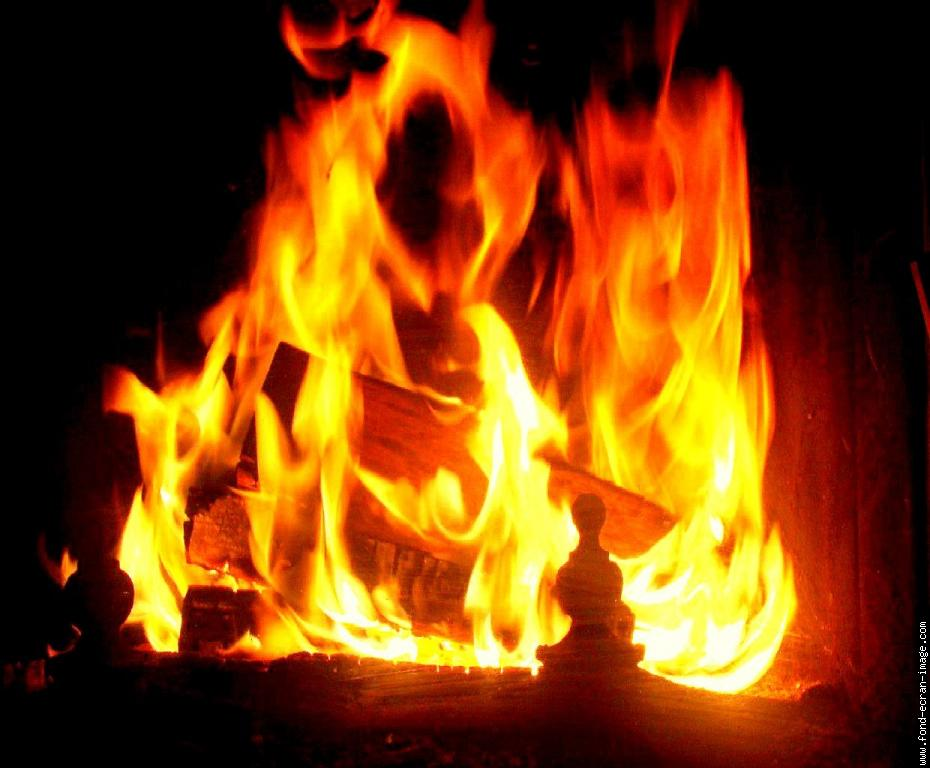
\includegraphics[scale=0.1]{feu.jpg}
  \end{figure}    
  \end{minipage}
  \begin{minipage}{0.48\linewidth}

  \begin{itemize}
    \item{Le feu}% flamme réaliste visuellement.
    \item{La fumée}% comportement réaliste.
    \item{Interactions avec des objets}% gérer les collisions entre le feu et les objets
    \item{Propagation du feu sur l'objet}% propagation du feu sur un objet
    \item{Combustion d'objet}% destruction de l'objet par le feu
  \end{itemize}
  \end{minipage}
  
\end{frame}

\begin{frame}{Les étapes de notre démarche}
  Découverte du milieu scientifique :
  \begin{itemize}
  \item{Apprendre une démarche de R\&D} % domaine de recherche
  \item{Étudier différents articles} % étude du sujet
  \item{Concevoir notre propre modèle} % comprehension des article et choix d'une solution
  \item{Implémenter le modèle} % sur CPU
  \item{Paralléliser le modèle en l'implémentant sur GPU} %
  \end{itemize}
\end{frame}


\section{Le modèle}
\begin{frame}{Le feu}
  \begin{itemize}
  \item Résultat de la combustion d'un fluide
  \item Le fluide se propage dans l'air
  \item La couleur de la flamme = f (chaleur, gaz)
  \end{itemize}
  \begin{figure}[!h]
    \centering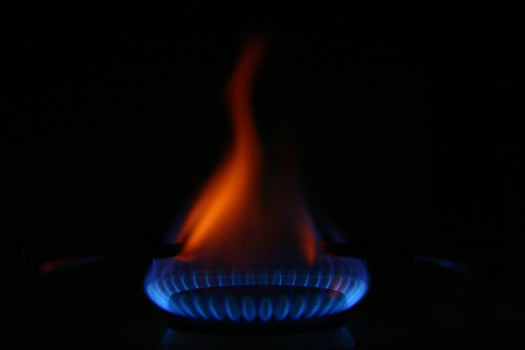
\includegraphics[scale=0.2]{Gaz.jpg}
    \caption{Gaz qui brûle}
    \label{Gaz}
  \end{figure}    
\end{frame}


\subsection{Le fluide}
\begin{frame}{Principe}
  \begin{itemize}
  \item Modèle basé sur le travail de \textbf{Jos Stam}, notamment
    \textbf{Stable Fluids}(SIGGRAPH 99 Conference Proceedings).
  \item Résolution de manière approchée des équation de Navier-Stokes
    pour la dynamique des fluides incompressibles.
  \end{itemize}
\end{frame}


\begin{frame}{Représentation du fluide}
  4 grilles uniformes 3D
  \begin{itemize}
    \item Densité de gaz ( flamme )
    \item Densité de fumée
    \item Temperature
    \item Champs de vitesse de l'air 
  \end{itemize}
\end{frame}



\begin{frame}{Phase 1 - La diffusion}
  Échange de valeurs avec les cases voisines.
  \begin{figure}[h]
    \centering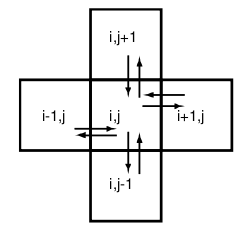
\includegraphics[scale=0.6]{STAM.png}
    \caption{Diffusion sur une grille 2D}
    \label{DiffusionStam}
  \end{figure}
\end{frame}


\begin{frame}{Phase 2 - Le transport}
  Déplacement des valeurs en fonction du champs de vitesse.
  \begin{figure}[h]
    \centering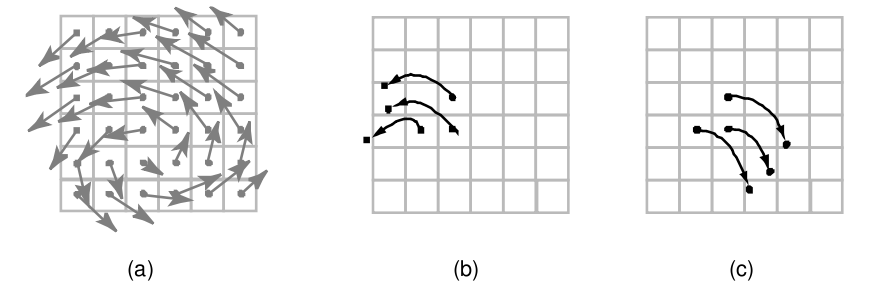
\includegraphics[scale=0.3]{STAM2.png}
    \caption{Résolution de l'advection par Backtracking introduite par \textbf{Jos Stam}}
    \label{AdvectionStam}
  \end{figure}
\end{frame}


\begin{frame}{}
  \begin{figure}[h]
    \centering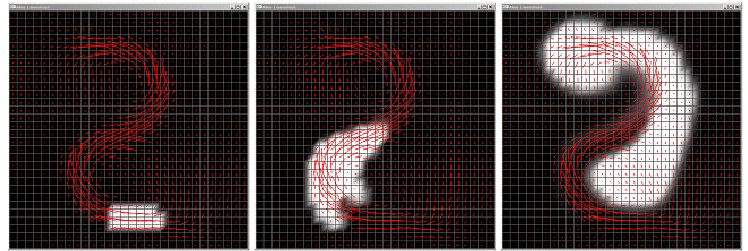
\includegraphics[scale=0.4]{Stam4.png}
    \caption{Advection d'une densité dans une grille 2D}
    \label{Bla}
  \end{figure}
\end{frame}



\begin{frame}{Phase 3 - La projection}
    But : avoir un fluide incomprésible\\
    Solution : gradient de la pression nul ( Décomposition de Hodge )\\
    Effet visuel : des vortex se créent\\
  \begin{figure}[h]
    \centering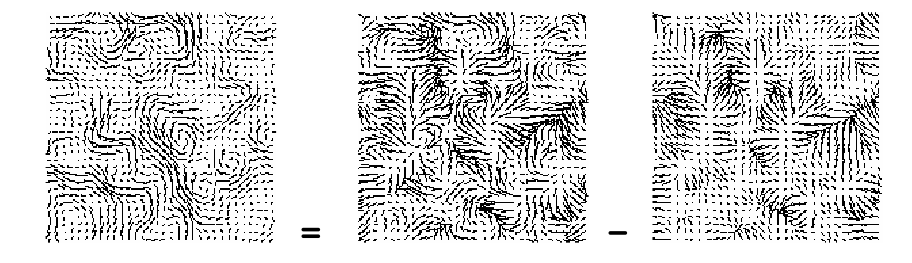
\includegraphics[scale=0.3]{STAM3.png}
    \caption{Correction du champ de vitesse par la soustraction du gradient}
    \label{ProjectionStam}
  \end{figure}
\end{frame}


\begin{frame}{Apéritif}
  \begin{figure}[h]
    \centering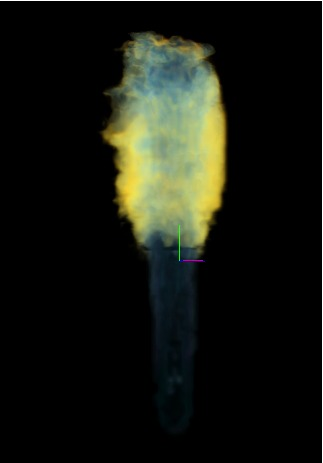
\includegraphics[scale=0.3]{FlammeBleue.jpg}
    \caption{Rendu de flamme sur la version finale}
    \label{ProjectionStam}
  \end{figure}
\end{frame}


\begin{frame}{Le rendu}
  Problème : tourner autour de l'image \\
  Solution : une texture 3D et une technique de ``billboard'',\\
             $\Rightarrow$ affichage de plans face à la camera \\
  \begin{minipage}{0.48\linewidth} 
    \begin{figure}[!h]
      \centering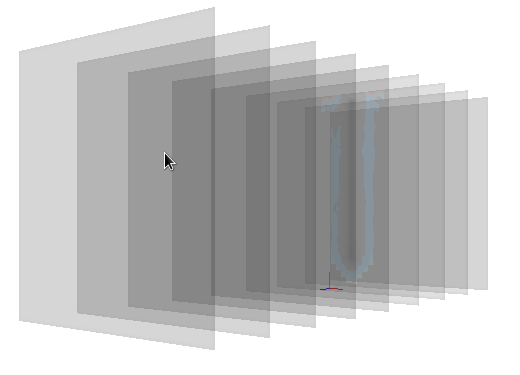
\includegraphics[scale=0.3]{Render3D.png}
      \caption{Vue des plans affichés}
      \label{PlanAffiche}
    \end{figure}
  \end{minipage}
  \begin{minipage}{0.48\linewidth}
    \begin{figure}[!h]
      \centering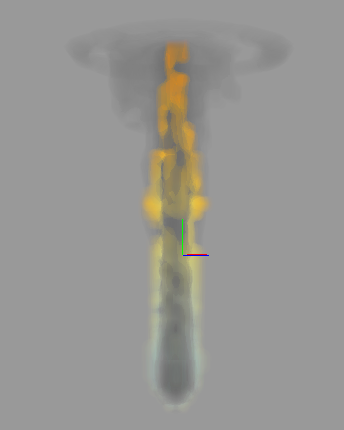
\includegraphics[scale=0.2]{Render3D3.png}
      \caption{Affichage normal face caméra}
      \label{VueFaceCam}
    \end{figure}
  \end{minipage}
  %image + perlin
\end{frame}


\begin{frame}{Coloration de la flamme}

  \begin{minipage}{0.48\linewidth} 
    \begin{figure}[!h]
      \centering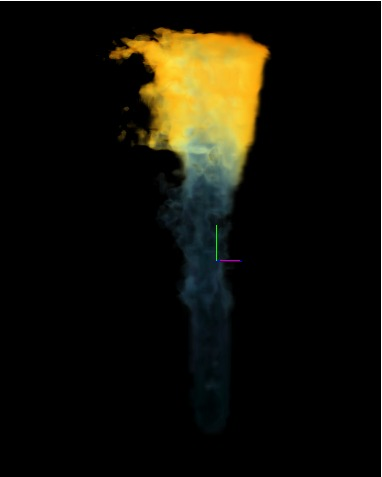
\includegraphics[scale=0.3]{FlammeBleue2.jpg}
      \caption{Coloration de la flamme}
      \label{PlanAffiche}
    \end{figure}
  \end{minipage}
  \begin{minipage}{0.48\linewidth}
  \begin{itemize}
  \item Corps noir
  \item Formule de Planck
  \end{itemize}
  \end{minipage}
\end{frame}

\begin{frame}{Bruit de perlin 4D}
  \begin{itemize}
  \item Bruit de perlin 3D lissé cosinusoïdalement
  \item Translation des coordonnées de texture
  \item Continuité temporelle
  \end{itemize} 
    \begin{figure}[!h]
      \centering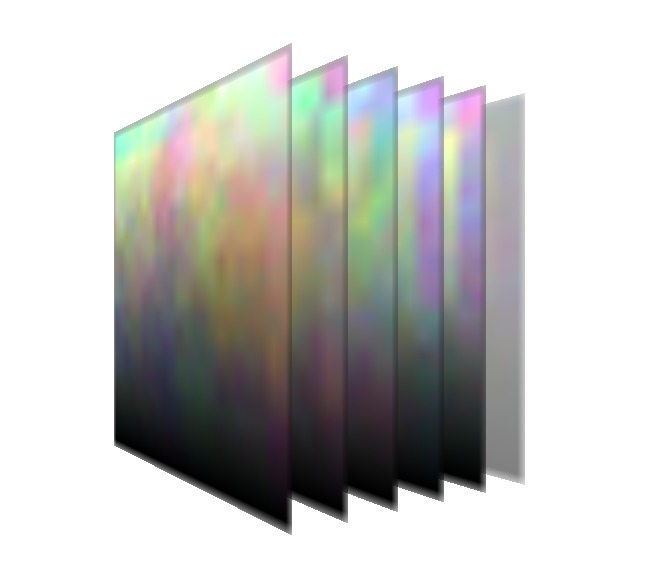
\includegraphics[scale=0.2]{Perlin3D.jpg}
    \end{figure}
\end{frame}

\begin{frame}{}
  \begin{minipage}{0.48\linewidth} 
    \begin{figure}[!h]
      \centering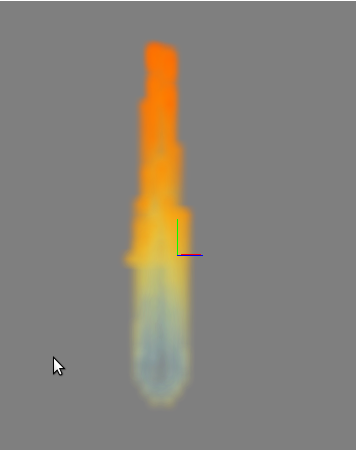
\includegraphics[scale=0.3]{SansPerlin.png}
      \caption{Sans le bruit de Perlin}
      \label{SansPerlin}
    \end{figure}
  \end{minipage}
  \begin{minipage}{0.48\linewidth}
    \begin{figure}[!h]
      \centering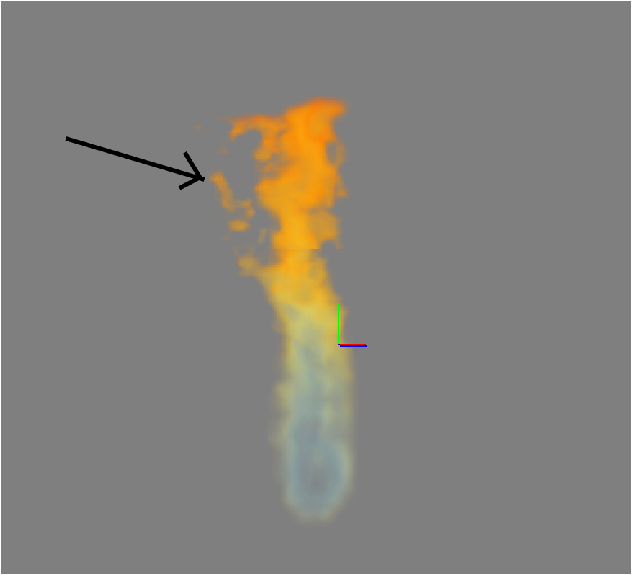
\includegraphics[scale=0.2]{Perlin1.png}
      \caption{Avec le bruit de Perlin}
      \label{AvecPerlin}
    \end{figure}
  \end{minipage}
\end{frame}

\begin{frame}
  \begin{center}
    \textbf{Entrée}
  \end{center}
\end{frame}



\subsection{Les objets}


\begin{frame}{Description des objets}
  \begin{itemize}
  \item Volumiques
  \item Différents matériaux
  \item Combustibles
  \item Température de combustion
  \end{itemize}
\end{frame}


\begin{frame}{Modèle d'intéraction}
  Interactions entre le modèle de fluide et le modèle d'objet.
  \begin{itemize}
  \item Présence des objets ( i.e. : pas de flamme a l'intérieur des objets )
  \item Transmission des informations de chaleur d'un modèle à l'autre.
  \item Gestion de la ``pyrolyse'' des objets.
  \end{itemize}
\end{frame}


\begin{frame}{Une représentation par voxel}
  Un objet $=$ un champ de voxels\\
  Interaction facilitée avec le modèle d'objet\\
  
  \begin{minipage}{0.48\linewidth} 
    \begin{figure}[!h]
    \centering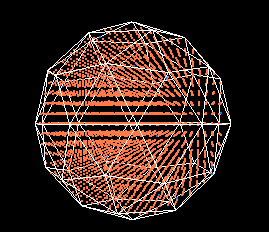
\includegraphics[scale=0.4]{Distance.png}
    \caption{Exemple de champ de distance}
      \label{SansPerlin2}
    \end{figure}
  \end{minipage}
  \begin{minipage}{0.48\linewidth}
    \begin{figure}[!h]
    \centering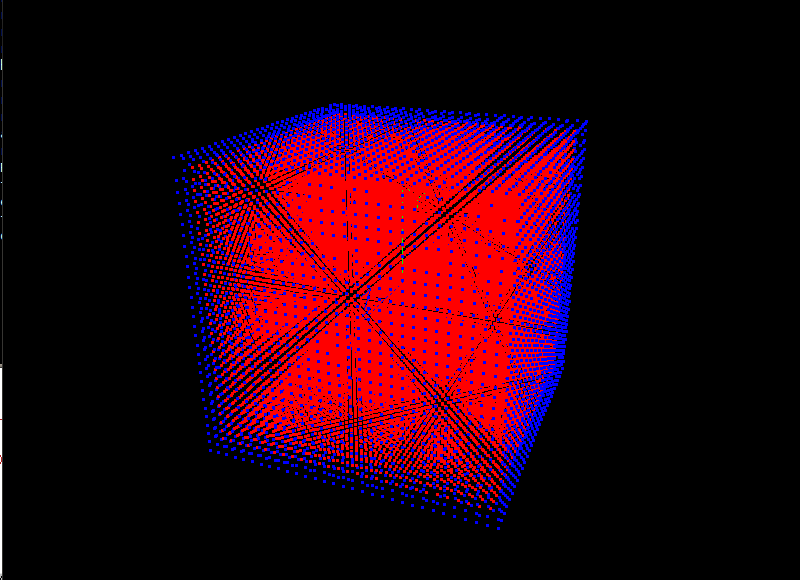
\includegraphics[scale=0.2]{phi_inside.png}
    \caption{Exemple de champ de distance 2}
      \label{AvecPerlin222}
    \end{figure}
  \end{minipage}
\end{frame}


\begin{frame}{Rendu}
  Besoin : recalculer la surface de l'objet localement.\\
  $\Rightarrow$ utilisation d'un algorithme de marching cube
  adaptatif.\\
  \begin{minipage}{0.48\linewidth} 
    \begin{figure}[!h]
      \centering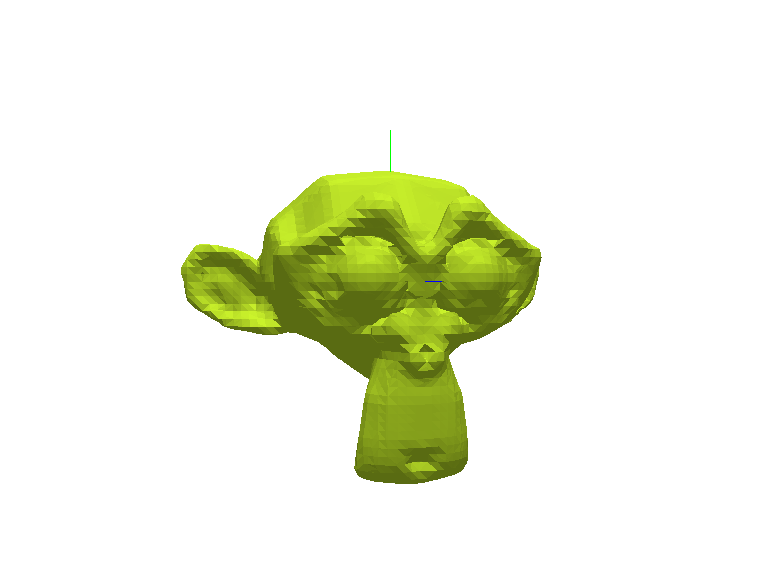
\includegraphics[scale=0.2]{FilledFace.png}
      \caption{Surface calculée par marching cube}
      \label{FilledFace}
    \end{figure}
  \end{minipage}
  \begin{minipage}{0.48\linewidth}
    \begin{figure}[!h]
      \centering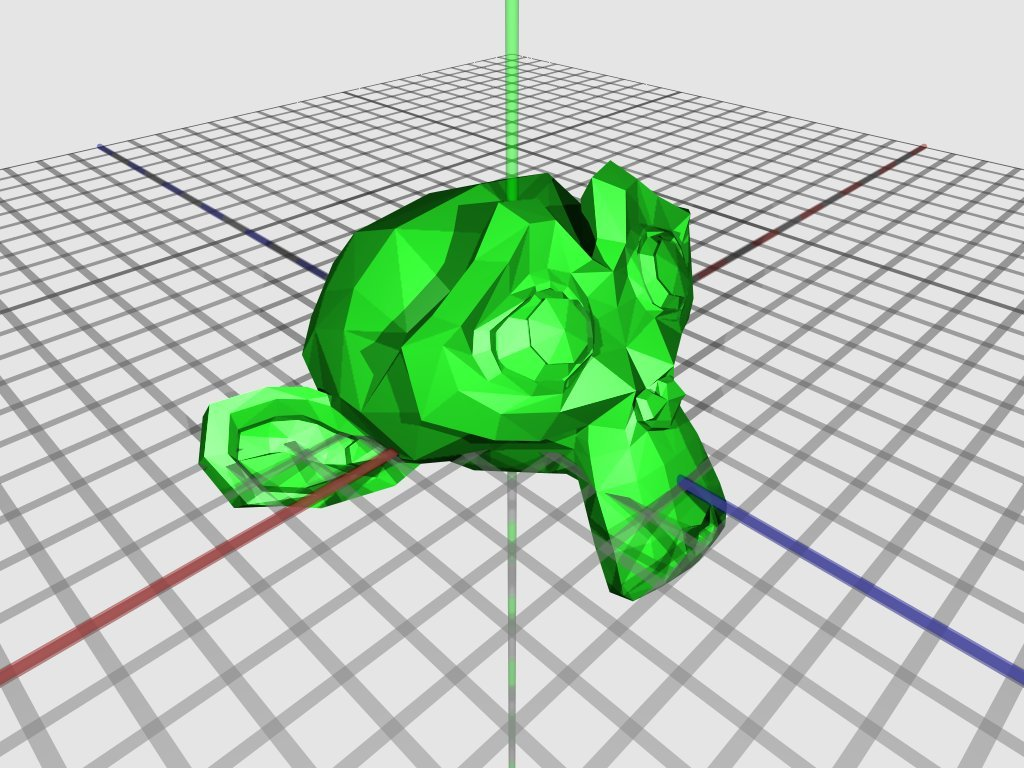
\includegraphics[scale=0.15]{Monkey.jpg}
      \caption{Mesh original}
      \label{LineFace}
    \end{figure}
  \end{minipage}
\end{frame}




\begin{frame}{Action des objets sur le fluide}
  Propagation du feu qui tient compte des objets\\
  $\Rightarrow$ champs de répulsion autour des objets.
  \begin{figure}[!h]
    \centering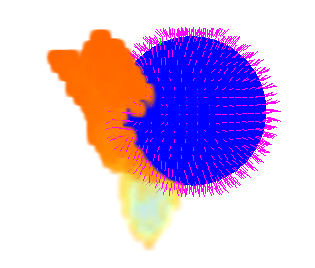
\includegraphics[scale=0.4]{Contour.png}
    \caption{Objet affiché avec son champs de répulsion}
    \label{repulsion}
  \end{figure}
\end{frame}


\begin{frame}{Combustion des objet}
    1 : combustion\\
    2 : génération de gaz / chaleur / fumée\\
    3 : si plus de matière : destruction du voxel et recalcul de la surface\\
  
  \begin{figure}[!h]
    \centering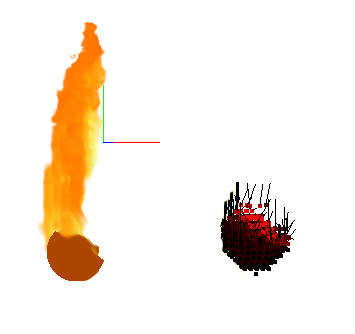
\includegraphics[scale=0.3]{Decomposition.png}
    \caption{Combustion d'une sphère, avec diffusion de la chaleur}
    \label{BoisQuiBrule}
  \end{figure}
\end{frame}

\begin{frame}
  \begin{center}
    \textbf{Plat principal}
  \end{center}
\end{frame}


\section{Portage du modèle de fluide sur GPU}
\begin{frame}{Le calcul sur GPU}
  Principe du modèle indentique, calcul différent.\\
  \begin{figure}[!h]
    \begin{tabular}{c|c|c}
       & CPU & GPU \\
      \hline
      données & tableau unidimentionnel  & texture 3D \\
      calcul  & itératif                 & parallèle par cellule \\
      rendu   & tableau vers texture 3D    & texture 3D \\
      coloration & function(chaleur) return RGB & couleur(texture 1D,chaleur) \\
      stockage & min 1E-37, max 1E+37 & min 0.0, max 1.0 \\
    \end{tabular}
  \end{figure}
\end{frame}


\begin{frame}{}
  \begin{figure}[!h]
    \centering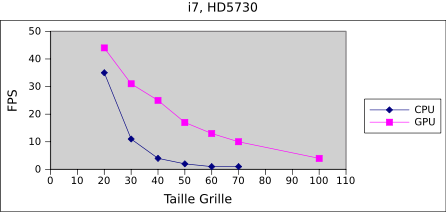
\includegraphics[scale=0.5]{Grille1.png}
    \caption{Comparatif de performances}
    \label{AvecPerlin33}
  \end{figure}
\end{frame}


\begin{frame}
  \begin{center}
    \textbf{Trou Normand}
  \end{center}
\end{frame}

\begin{frame}{Problème rencontré}
  \begin{itemize}
  \item dessin dans un \textbf{frame buffer}
  \item calculs fait par le \textbf{fragment shader}
  \end{itemize}
  \begin{figure}[!h]
    \centering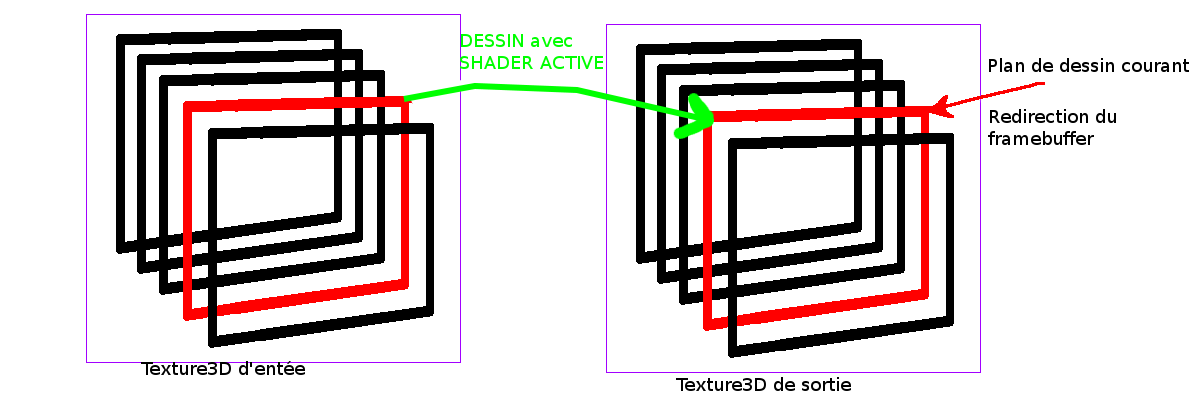
\includegraphics[scale=0.25]{Framebuffer.png}
    \caption{Frame Buffer Object}
    \label{AvecPerlin}
  \end{figure}
\end{frame}


\section{Démonstration}
\begin{frame}
  \begin{center}
    \textbf{Dessert}
  \end{center}
\end{frame}

\section{Conclusion}
\begin{frame}{Conclusion}
  \begin{itemize}
  \item Résultats très satisfaisants
  \item Modèle complet
  \item Beaucoup de nouvelles connaissances
  \item Petite déception pour le GPU
  \end{itemize}
\end{frame}

\begin{frame}{Remerciements}
  \begin{itemize}
  \item{Marie-Paule Cani} pour avoir accepté de nous encadrer, pour
    ses conseils et indices de recherche.
  \item{Cyril Crassin} pour nous avoir aidé à comprendre le
    fonctionnement de GLSL.
  \item{Aurelie Catel} pour le suivi de gestion de projet.
  \item{Nintendo\texttrademark} pour Super Smash Bross Melee ©.
  \end{itemize}
\end{frame}

\end{document}

